The first step is to compare the performance of Apache and Nginx web serving software. However, it is not necessary to compare these software in their speed of serving static content (for example HTML files) because it has been proven and because of Nginx architecture that Nginx is more performant in this manner.

What is interesting to compare, though, is running of PHP under Apache and Nginx.

\section{Apache with mod\_php}

"Apache supports a variety of features, many implemented as compiled modules which extend the core functionality." "Instead of implementing a single architecture, Apache provides a variety of MultiProcessing Modules (MPMs), which allow Apache to run in a process-based, hybrid (process and thread) or event-hybrid mode, to better match the demands of each particular infrastructure." \cite{Apache:Wiki}\\

In a default configuration, when HTTP requests are received, Apache starts to process them one by one. It spawns multiple child processes to handle the load. However, these proccesses are standalone, meaning they initialize all modules (including mod\_php) even for static file requests. This behavior results in high RAM usage as seen on figure \ref{fig:apache_mod_php}. \\

mod\_php is a PHP interpreter module for Apache. It is the most common way of executing PHP scripts when using Apache HTTP. The module is loaded in each Apache process, thus a request for a PHP script is executed directly within the process, not being relayed to another server with the ability to run the script. The main disadvantage to embedding PHP inside Apache is that if a user is requesting a static resource such as CSS, JS or an image, it still has to go through Apache process with PHP module, therefore increasing RAM and CPU usage.

\subsection{Load testing Apache with mod\_php}

We are going to load test Apache with mod\_php running a simple WordPress-powered site. Within your command line, navigate to the wordpress-ansible directory and run the "apache\_mod\_php.yml" Ansible playbook:


\begin{lstlisting}
ansible-playbook -i hosts apache_mod_php.yml
\end{lstlisting}

The playbook will configure Apache and create a virtual host for the WordPress site. We are using a default Apache HTTP configuration file without any performance modifications. \cite{WP_Ansible:apache.conf}\\

To deploy the simple WordPress site, run the "wordpress\_basic.yml" Ansible playbook. It will download the latest version of WordPress with the default theme and installs the database tables. We are now ready to carry out the testing. \\

At the loader.io load testing service, we have created a new test \cite{Loader.io:apache_mod_php}, configuring it to send from 0 to 200 simultaneous client requests to the index of our testing server for a duration of 30 seconds. Figure \ref{fig:apache_mod_php} depicts the final chart.


\begin{figure}[H]
\begin{center}
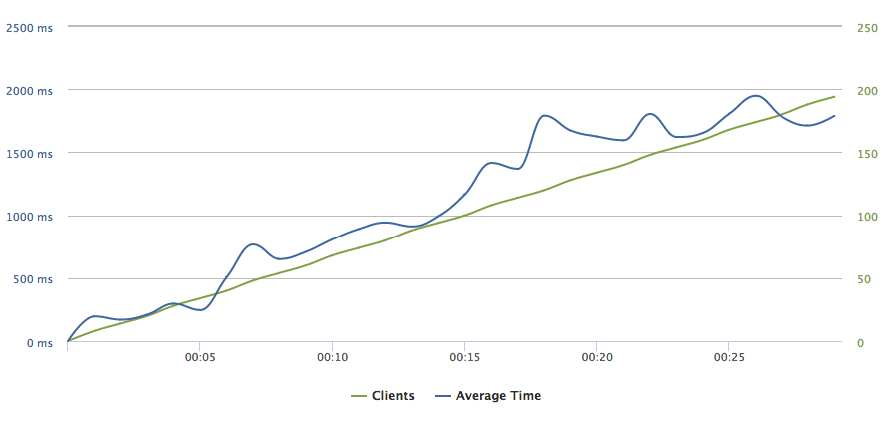
\includegraphics[scale=0.5]{figures/Apache_mod_php.png}
\caption{Apache HTTP with mod\_php: clients versus average response time}
\label{fig:apache_mod_php}
\end{center}
\end{figure}

This chart shows the average server response times when a number of simultaneous client requests are sent to it. We can observe that even under a high load of 200 concurrent requests the average response time is under 2 seconds. It grows approximately linearly. \\

However, to truly see how the server copes with the load, the figures \ref{fig:apache_mod_php_2s} and \ref{fig:apache_mod_php_25s} come in handy. They represent screenshots of Htop interactive process viewer \cite{Htop:main_site} during 2 and 25 seconds into the load testing, respectively.

\begin{figure}[H]
\begin{center}
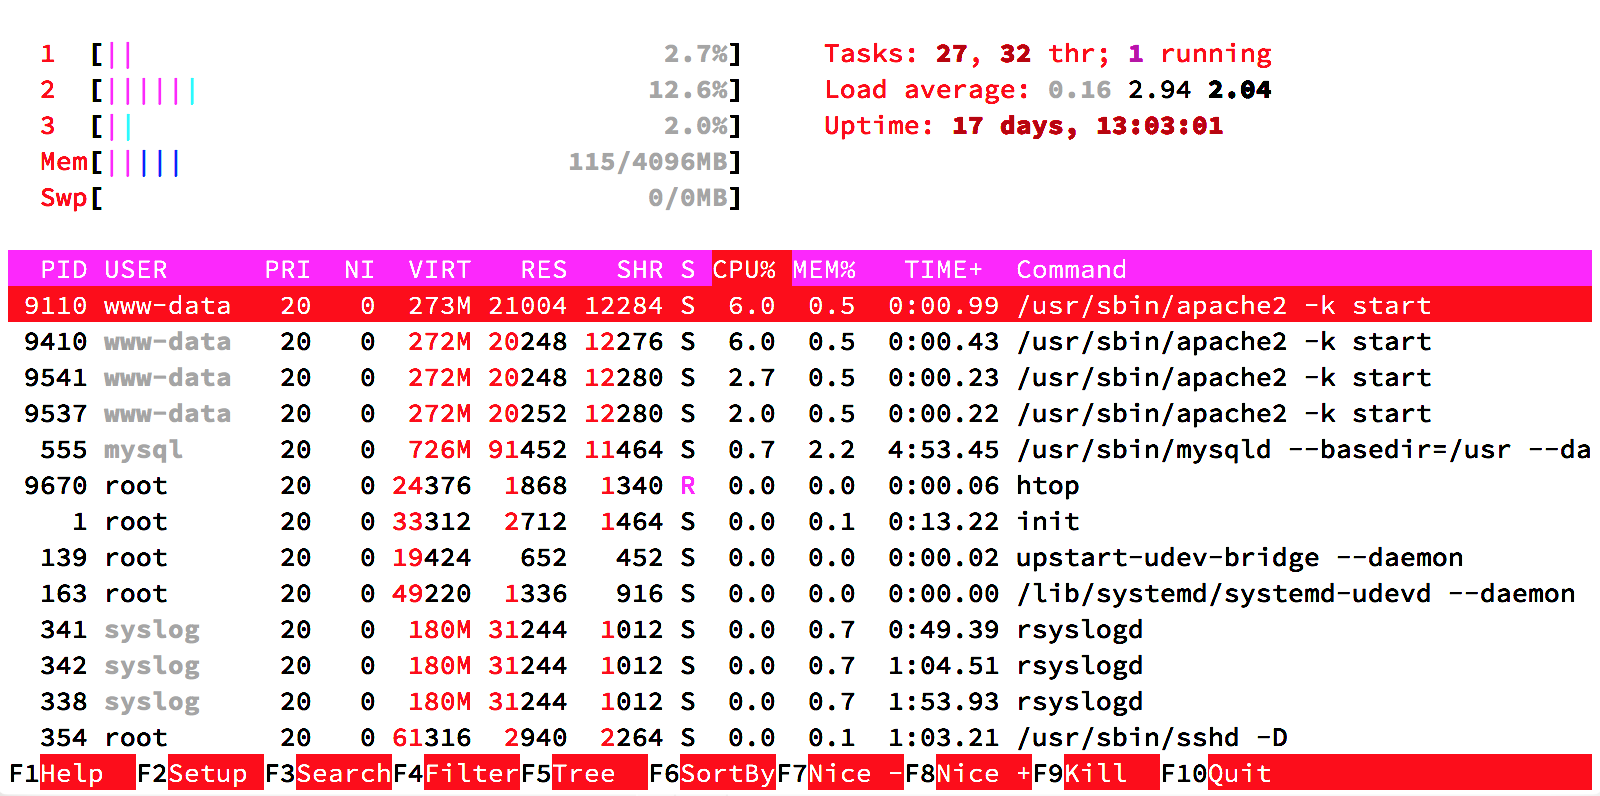
\includegraphics[scale=0.5]{figures/Apache_mod_php_2s.png}
\caption{Apache HTTP with mod\_php: Htop process viewer 2 seconds into test}
\label{fig:apache_mod_php_2s}
\end{center}
\end{figure}

On the screenshot, we can see a table of currently running processes. The columns RES, CPU\% and MEM\% show the RAM usage in kilobytes, CPU usage in percentage and RAM usage in percentage of a process, respectively. What is more, there are several gauges, visually depicting the usage or particular CPU core (or thread), RAM and Linux Swap. Opening the Htop's help screen (F1 in Htop), the gauges are explained as follows:

\begin{figure}[H]
\begin{center}
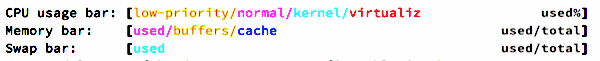
\includegraphics[scale=0.5]{figures/htop_help_gauges.png}
\caption{Screenshot of Htop's help screen explaining the main gauges}
\label{fig:htop_help_gauges}
\end{center}
\end{figure}

It is crucial to notice that the yellow bars in the Memory bar section show cached memory, which is not counted towards the used memory since it can be misleading at times (will discuss this a bit later).

\begin{figure}[H]
\begin{center}
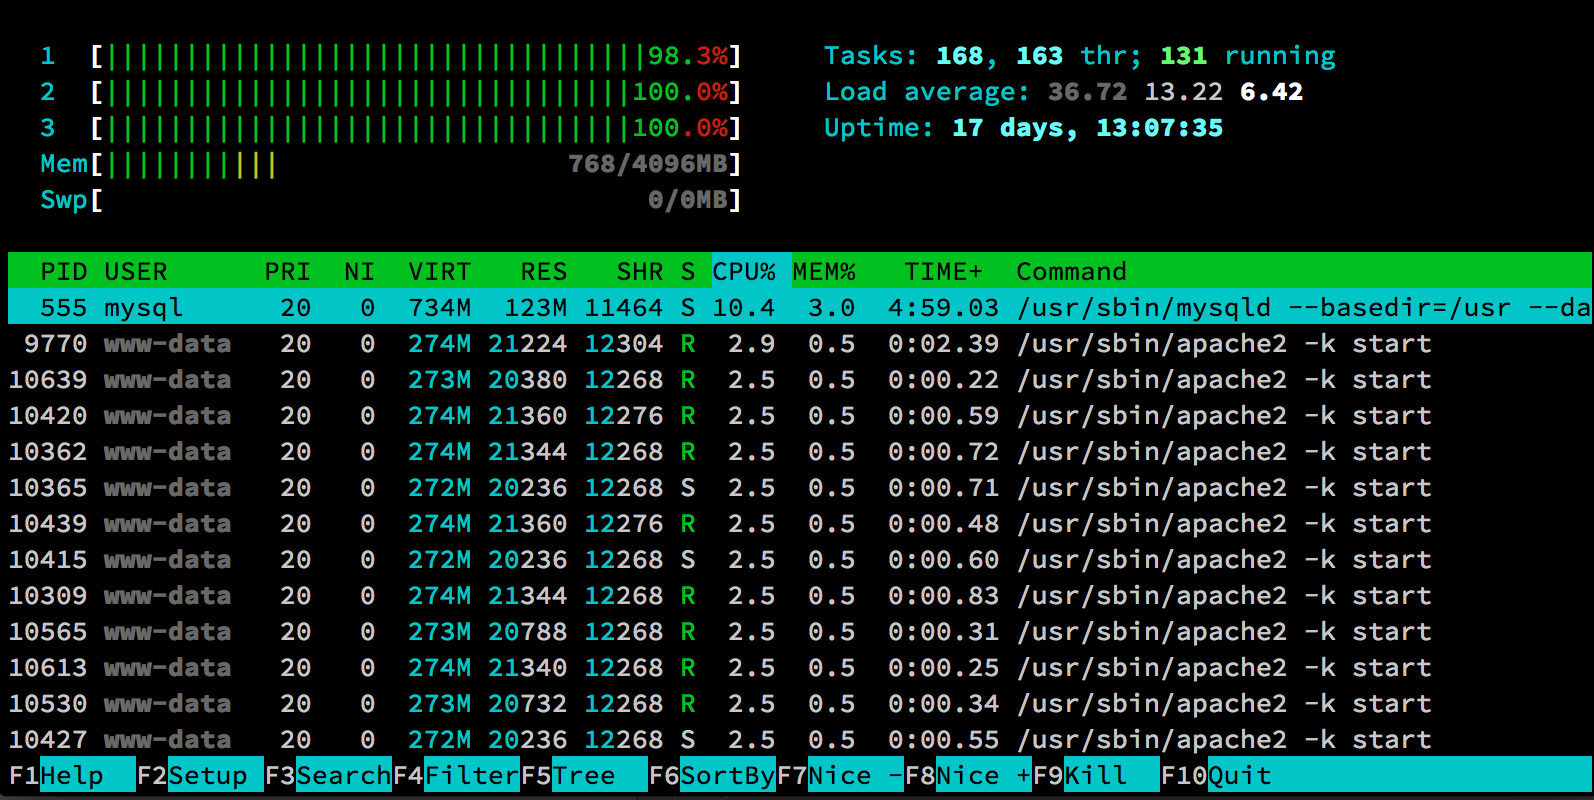
\includegraphics[scale=0.5]{figures/Apache_mod_php_25s.png}
\caption{Apache HTTP with mod\_php: Htop process viewer 25 seconds into test}
\label{fig:apache_mod_php_25s}
\end{center}
\end{figure}

From both screenshots, we can observe that Apache HTTP, represented by the process /usr/sbin/apache2 is, at first, just warming up, spawning three child processes and under heavy load, consuming the CPU completely and taking about 770 megabytes of memory. It does not tell us much without comparing it to the results of benchmarking different server stacks, what we are going to do shortly. \\

Loader.io testing results page \cite{Loader.io:apache_mod_php} also shows us more statistics about the test:

\begin{itemize}
	\item\textbf{Average response time:} 1229 ms
	\item\textbf{Min/Max response times:} 144 / 4660 ms
	\item\textbf{Count of successful responses:} 2178
\end{itemize}

\section{Nginx with PHP-FPM}

Nginx has an event-based architecture. It means that when an request arrives, Nginx asynchronously listens for it. Then when it arrives, it is processed asynchronously. The main usage for Nginx is to quickly process many requests, relaying them to other applications if they need to be processed further. That's why we need to use PHP-FPM.

PHP-FPM is a FastCGI server bound to a TCP port or socket. It listens for PHP requests, processing them and outputting the rendered content.

When using Ningx with PHP, we have to detect if the request is for a PHP file. If it is, we need to redirect the request into the PHP-FPM server, waiting for the reply which is then outputted as a response.


To compare Apache with mod\_php and Nginx with PHP-FPM, they are similarly performant. Apache + mod\_php can achieve better performance at the expense of wasting more resources as it has to spawn a large number of threads to process more requests. 

\begin{figure}[H]
\begin{center}
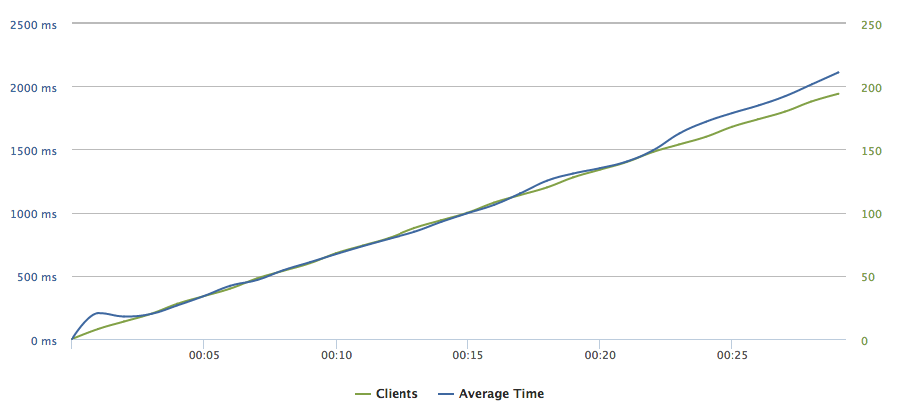
\includegraphics[scale=0.5]{figures/Nginx_PHP-FPM.png}
\caption{Nginx with PHP-FPM: clients versus average response time}
\label{fig:nginx_php-fpm}
\end{center}
\end{figure}

\begin{figure}[H]
\begin{center}
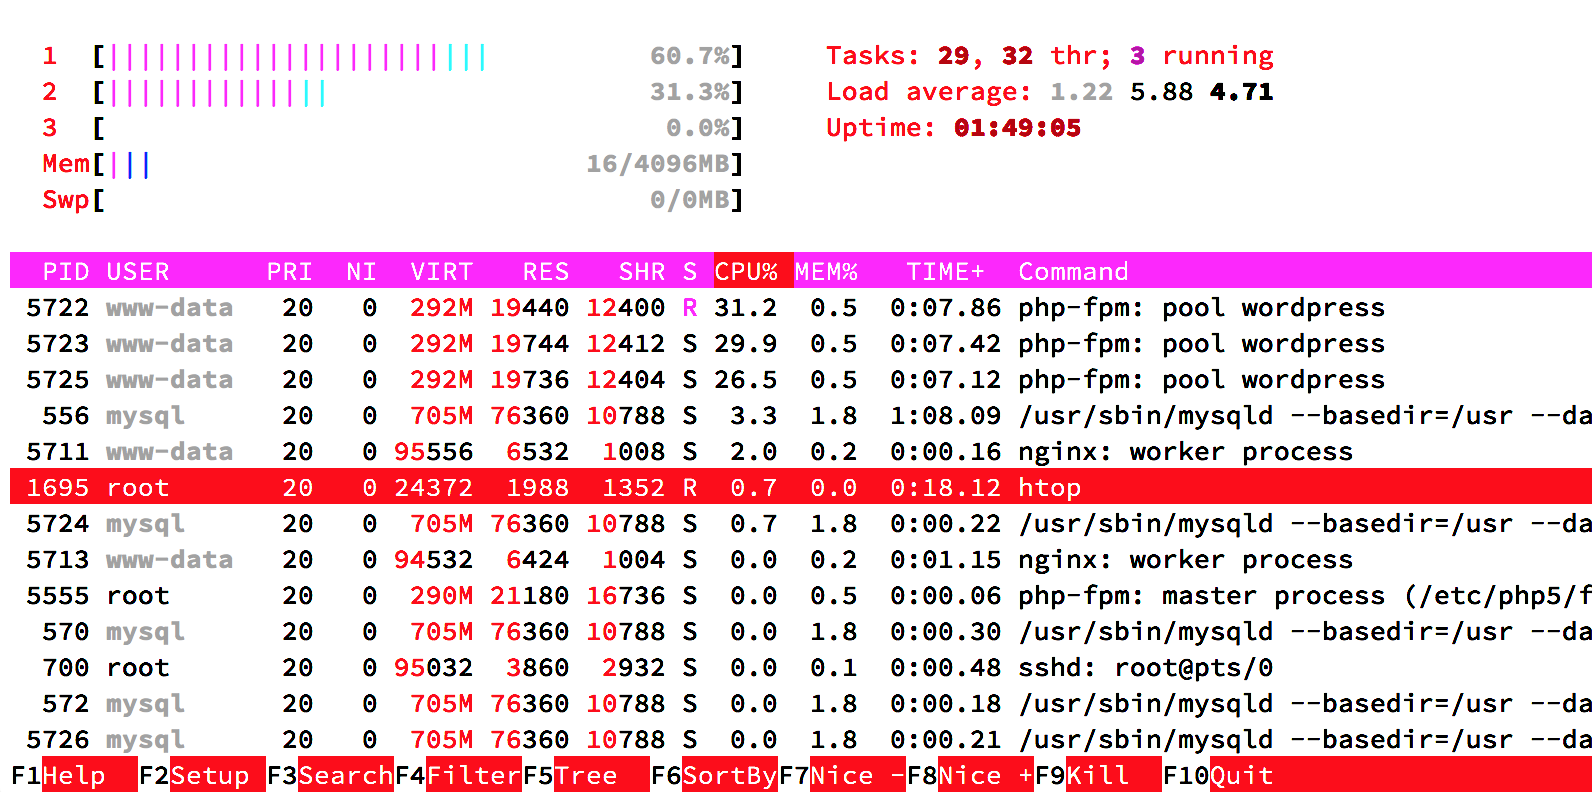
\includegraphics[scale=0.5]{figures/Nginx_PHP-FPM_1s.png}
\caption{Nginx with PHP-FPM: Htop process viewer 1 second into test}
\label{fig:nginx_php-fpm_1s}
\end{center}
\end{figure}

\begin{figure}[H]
\begin{center}
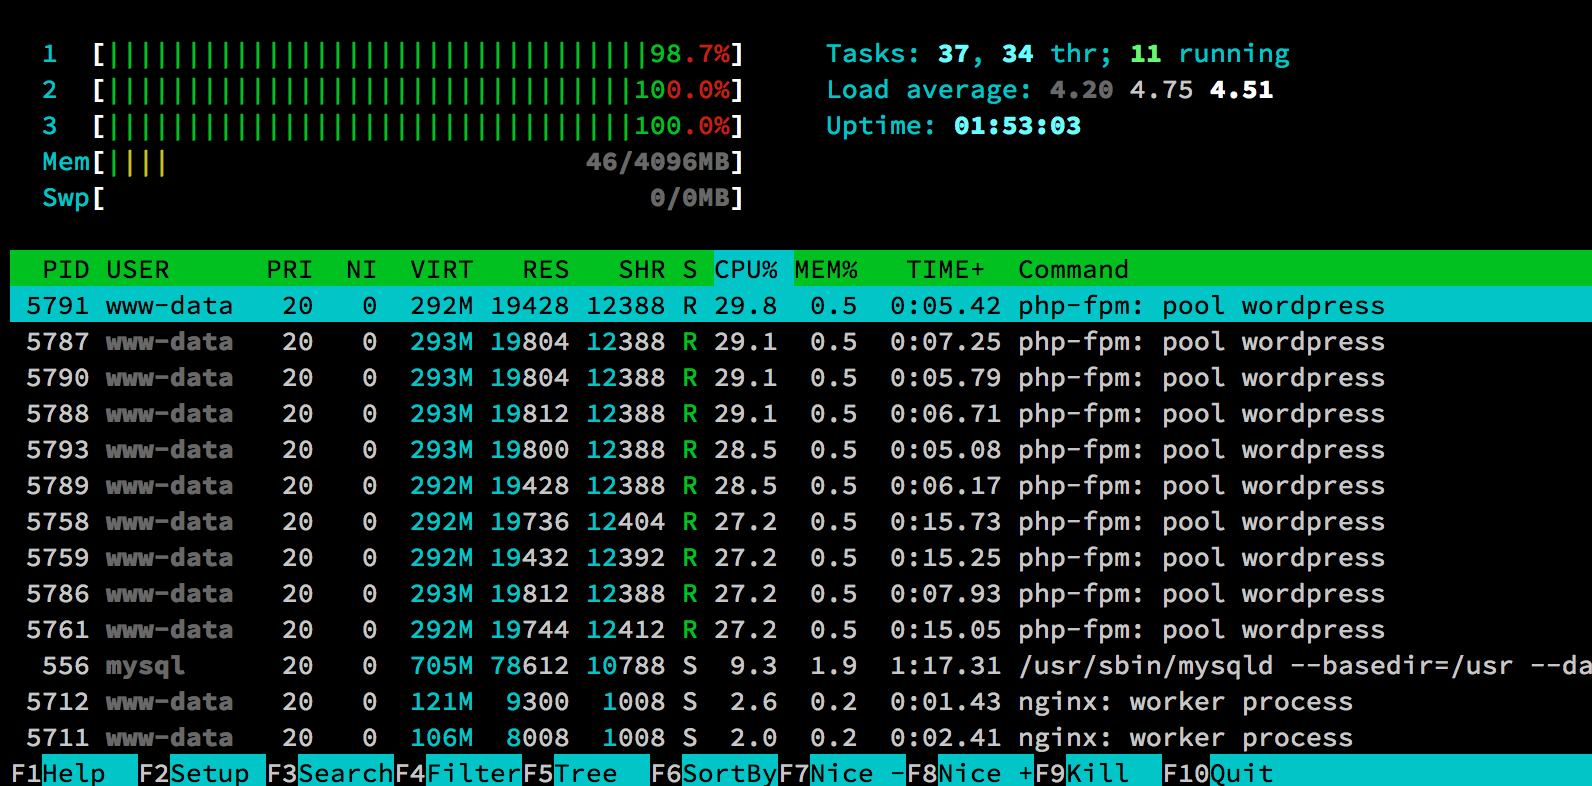
\includegraphics[scale=0.5]{figures/Nginx_PHP-FPM_22s.png}
\caption{Nginx with PHP-FPM: Htop process viewer 22 seconds into test}
\label{fig:nginx_php-fpm_22s}
\end{center}
\end{figure}

Avid readers will notice that the RAM usage by MariaDB is higher than the total ram usage.

\section{Nginx + HHVM}

In the previous section, we have seen the performance of Nginx + PHP-FPM. Now, we will compare it with Nginx using HHVM for PHP processsing.

"HipHop Virtual Machine (HHVM) is a process virtual machine based on just-in-time (JIT) compilation, serving as an execution engine for PHP...". "By using the principle of JIT compilation, executed PHP or Hack code is first transformed into intermediate HipHop bytecode (HHBC), which is then dynamically translated into the x86-64 machine code, optimized and natively executed.[1][4] This contrasts to the PHP's usual interpreted execution, in which the Zend Engine transforms the PHP source code into opcodes as a form of intermediate code, and executes the opcodes directly on the Zend Engine's virtual CPU".

It is developed by Facebook with source code hosted on GitHub (open source).

\begin{figure}[H]
\begin{center}
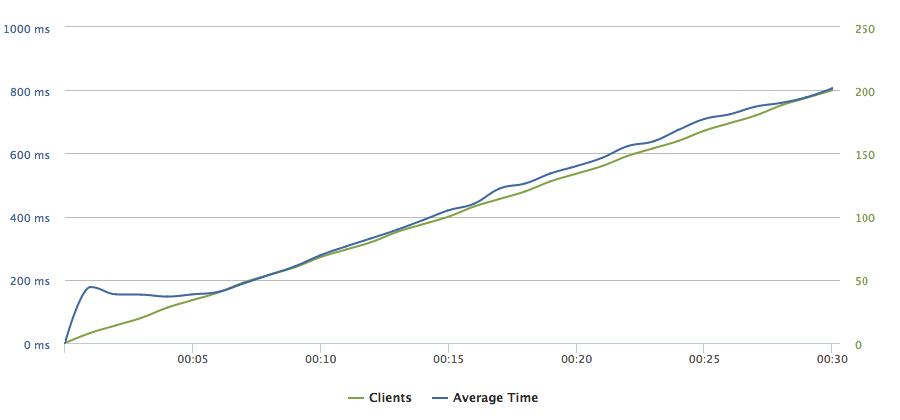
\includegraphics[scale=0.5]{figures/Nginx_HHVM.png}
\caption{Nginx with HHVM: clients versus average response time}
\label{fig:nginx_hhvm}
\end{center}
\end{figure}

\begin{figure}[H]
\begin{center}
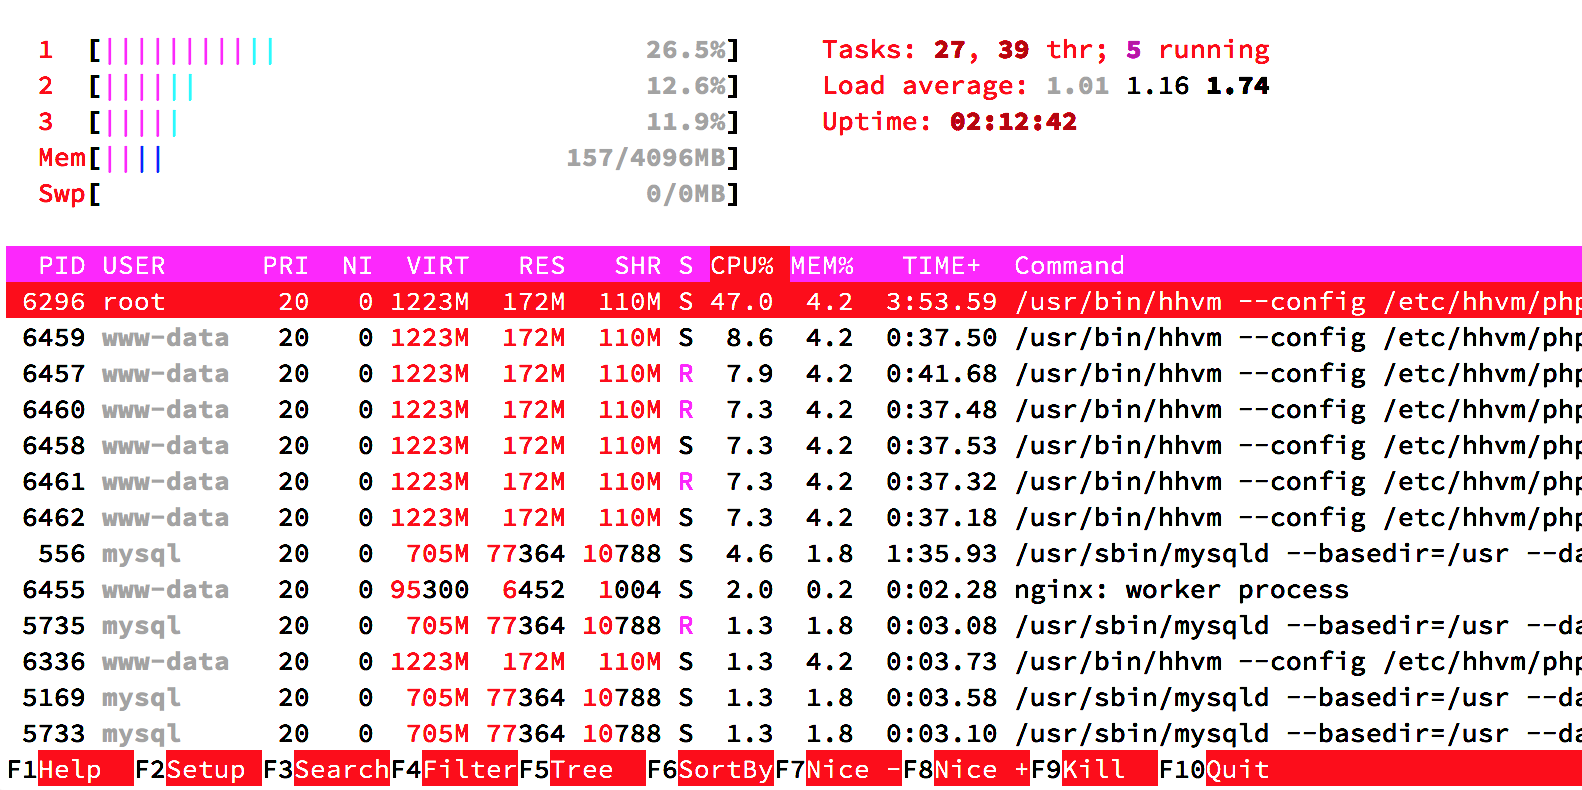
\includegraphics[scale=0.5]{figures/Nginx_HHVM_1s.png}
\caption{Nginx with HHVM: Htop process viewer 1 second into test}
\label{fig:nginx_hhvm_1s}
\end{center}
\end{figure}

\begin{figure}[H]
\begin{center}
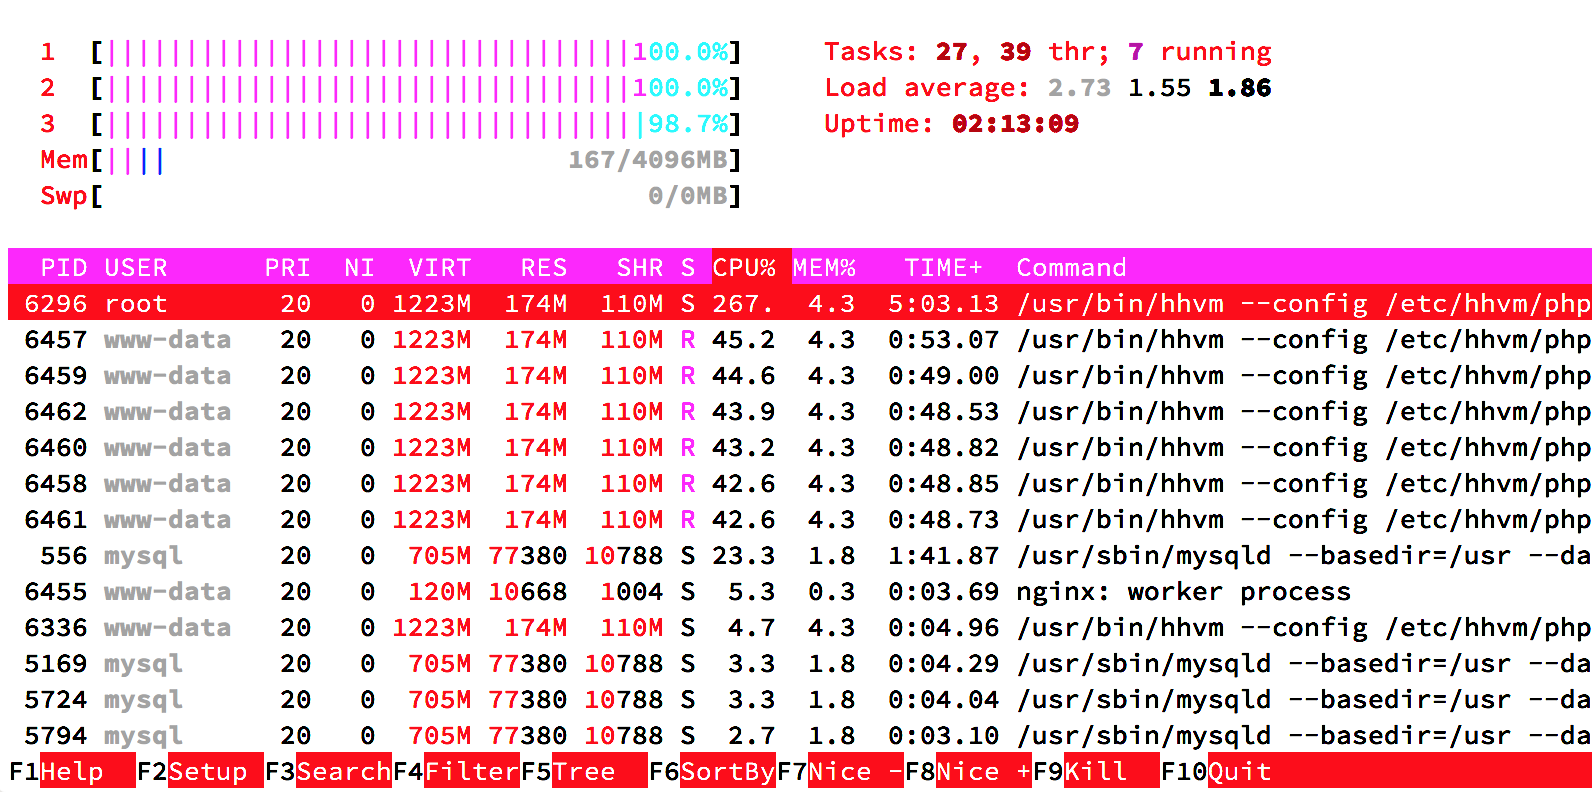
\includegraphics[scale=0.5]{figures/Nginx_HHVM_24s.png}
\caption{Nginx with HHVM: Htop process viewer 22 seconds into test}
\label{fig:nginx_hhvm_24s}
\end{center}
\end{figure}

As we can see, HHVM has much better performance profile. It can handle more requests, with less RAM usage and CPU usage. The best combination as your web serving software. 

Much higher throughput of successful requests.